\documentclass{article}

% Language setting
% Replace `english' with e.g. `spanish' to change the document language
\usepackage[portuguese]{babel}

\usepackage{subfig}

% Set page size and margins
% Replace `letterpaper' with `a4paper' for UK/EU standard size
\usepackage[letterpaper,top=3cm,bottom=2cm,left=3cm,right=2cm,marginparwidth=1.75cm]{geometry}

% Useful packages
\usepackage{amsmath}
\usepackage{graphicx}
\usepackage[colorlinks=true, allcolors=black]{hyperref}

\title{Relatório do EP de MAC0209}
\author{
    Antonio Fernando Silva e Cruz Filho\\
    Cássio Azevedo Cancio\\
    Eduardo Mendes Lopes\\
    Guilherme Mota Pereira\\
    Larissa Vitoria Medeiros Silva\\
    Luiz Gabriel Lima Arrais
}

\begin{document}
\maketitle


\begin{abstract}
\quad Esse exercício-programa foi feito para a matéria de Modelagem e Simulação. O trabalho foi dividido em duas partes: na primeira, o objetivo era utilizar uma plataforma de coleta de imagens de ruas e rodovias, Kartaview, para fazer a análise de diferentes métodos de medição de distância e compará-los. Na segunda parte, foi necessário fazer a modelagem de diferentes movimentos. O grupo escolheu analisar o Bloco na Rampa e o Movimento Circular.
\end{abstract}

\newpage

\tableofcontents

\newpage

\section{Cronograma}

\subsection{Gantt Chart}

\begin{center}
\frame{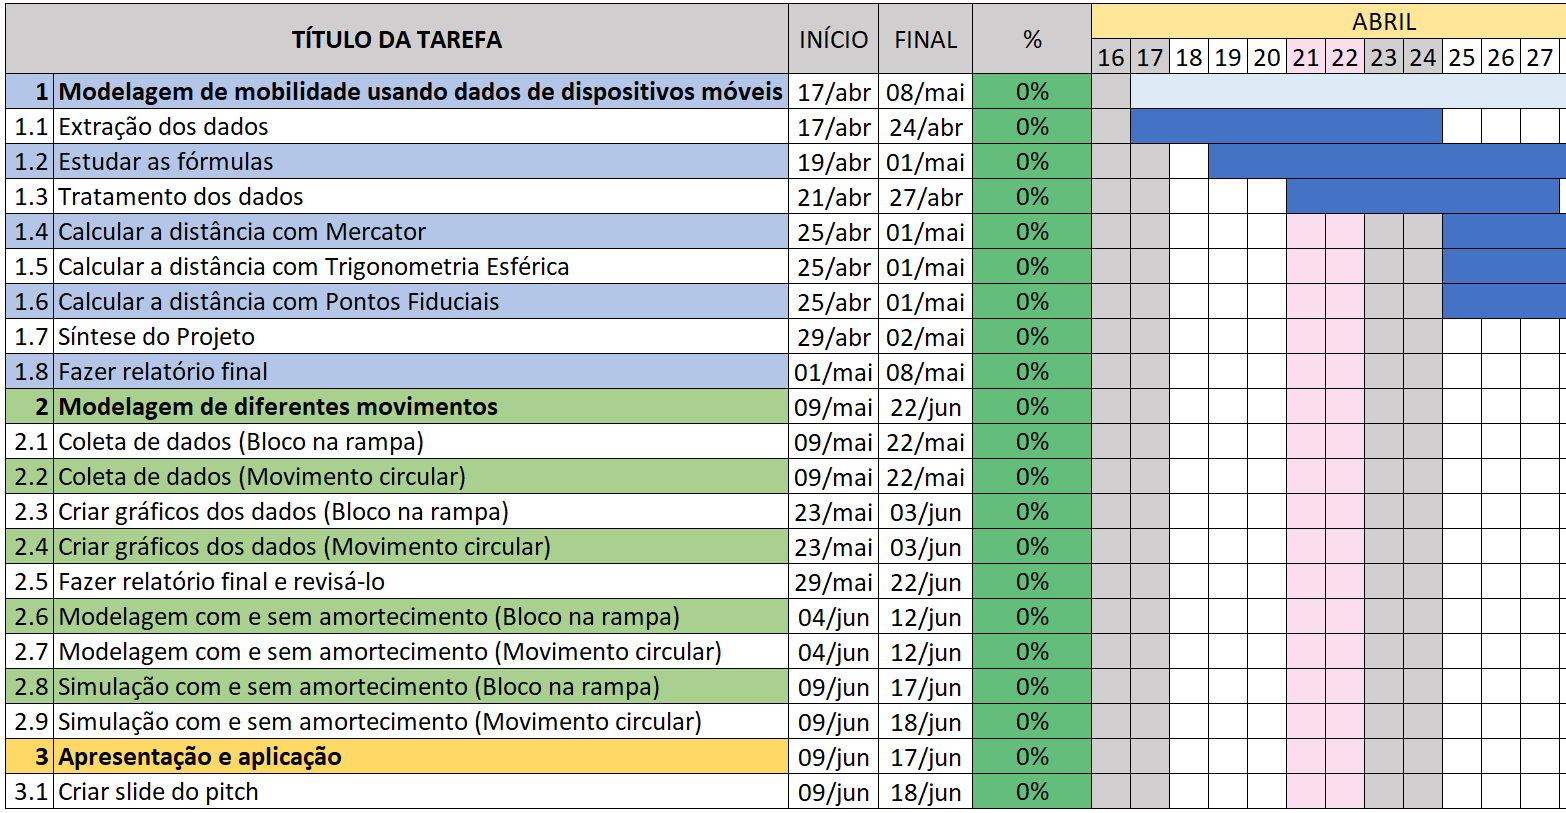
\includegraphics[width=13cm]{./img/Parte 1.png}}\\
\frame{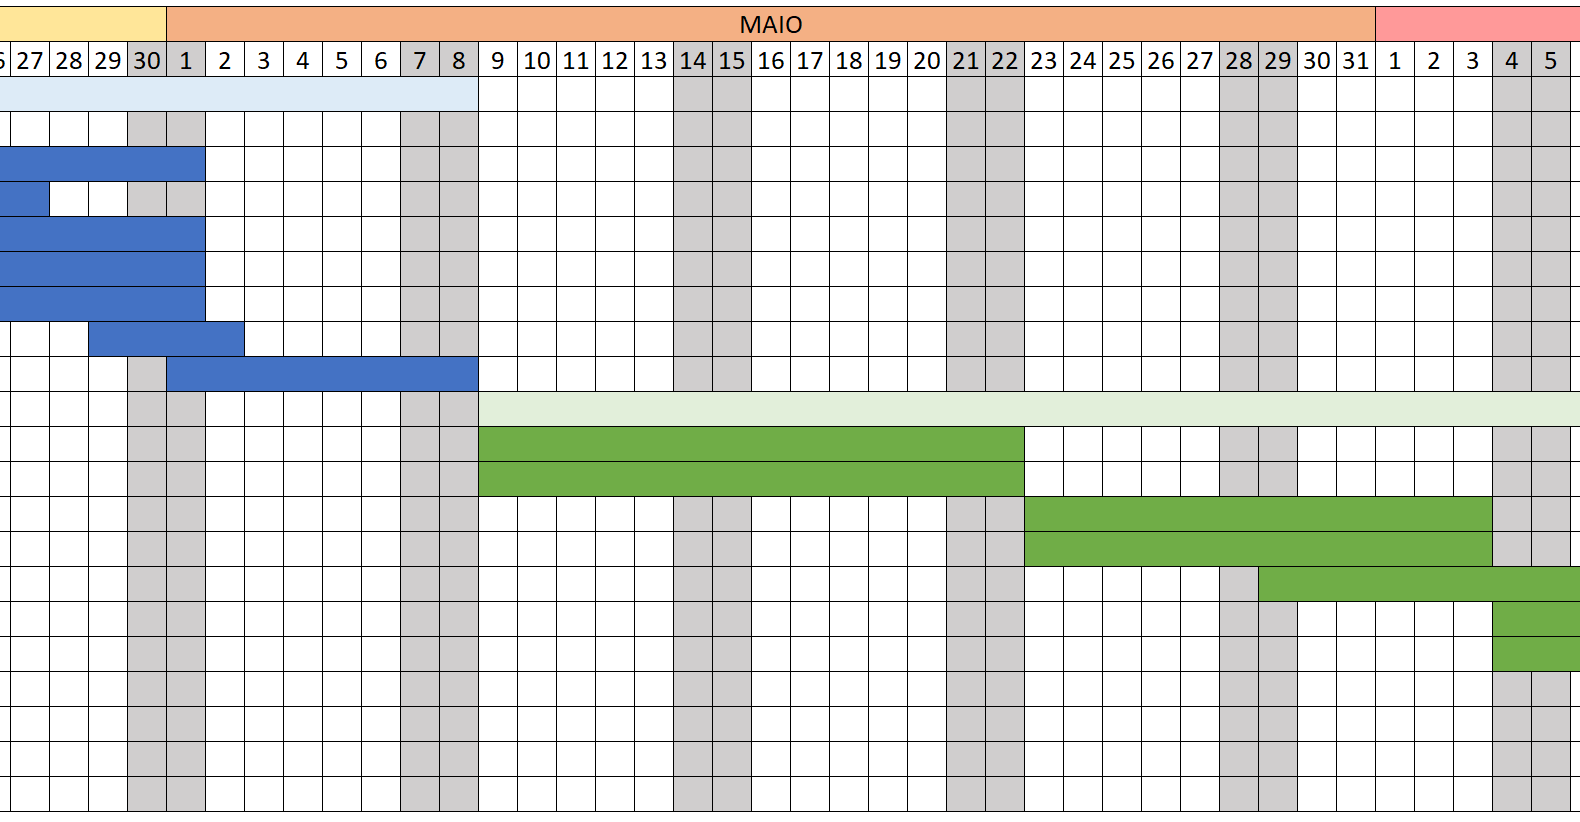
\includegraphics[width=13cm]{./img/Parte 2.png}}\\
\frame{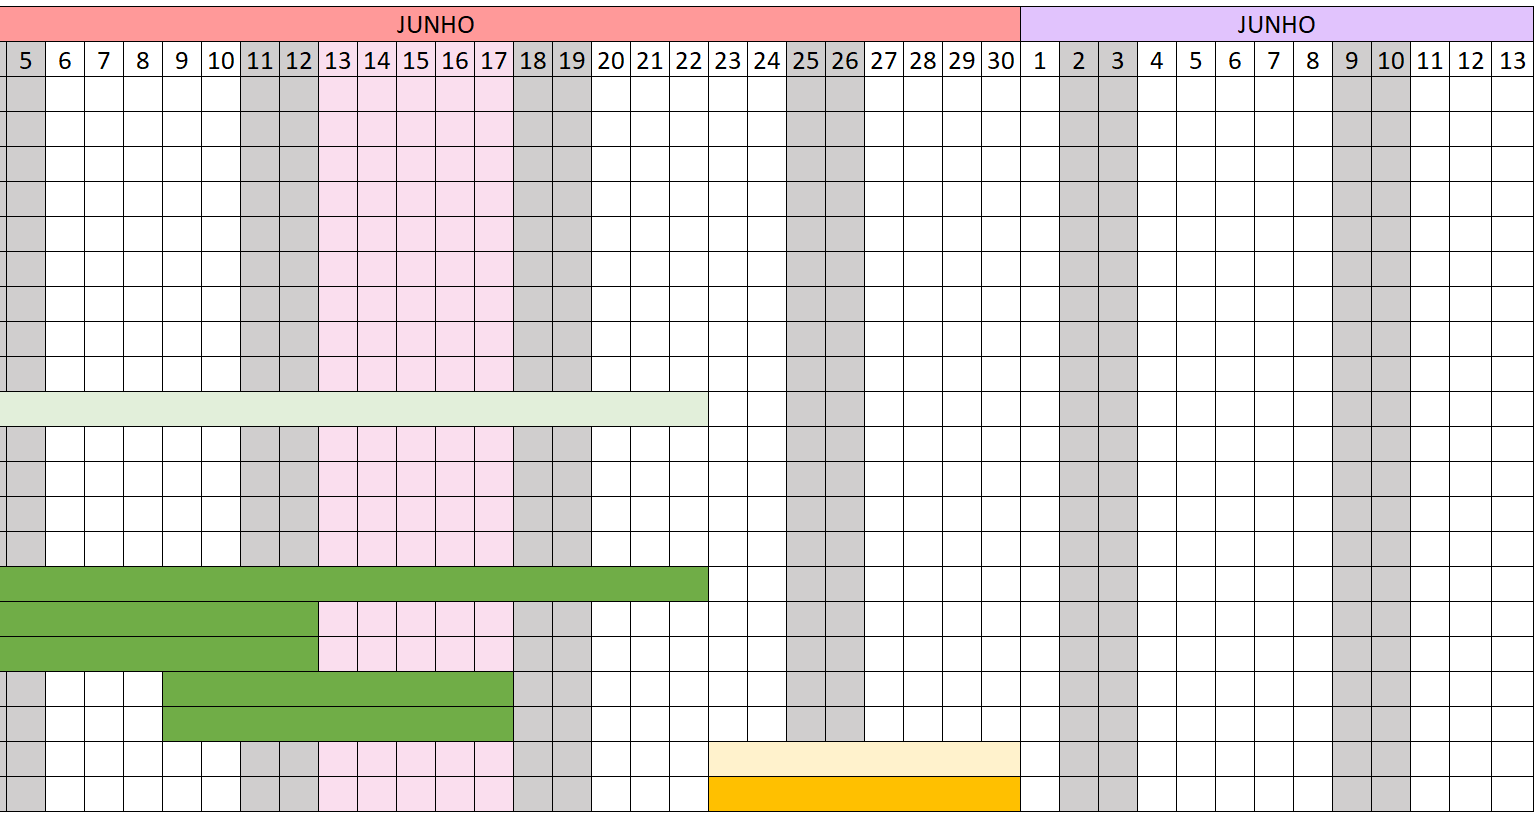
\includegraphics[width=13cm]{./img/Parte 3.png}}
\end{center}

\section{Kartaview}

\subsection{Introdução}

\qquad Primeiramente, foi necessário escolher duas rodovias, uma no Brasil e outra no exterior, para que os métodos desenvolvidos pudessem ser testados. Basicamente, o Kartaview disponibiliza fotos retiradas por um celular em algum trajeto percorrido por um usuário da plataforma de carro. O grupo decidiu utilizar, para o trecho nacional, um pedaço da rodovia SP-248 próximo à cidade do Guarujá, em São Paulo, já o trecho no exterior, foi a rodovia M6 no Reino Unido, próximo à vila de Old Hutton em South Lakeland.

\begin{figure}[!h]
    \centering
    \subfloat[Guarujá]{{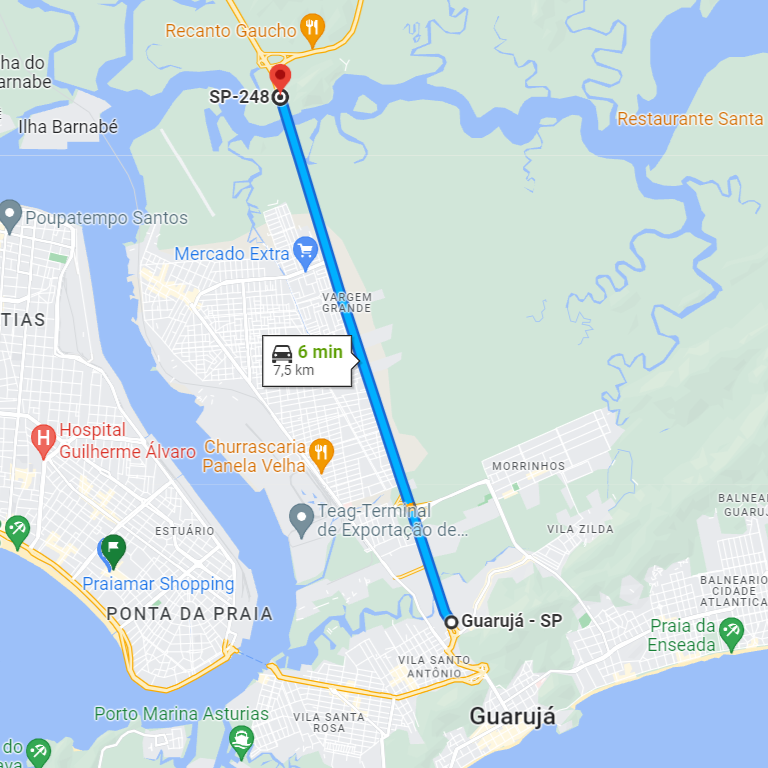
\includegraphics[width=6cm]{./img/mapaGuaruja.png} }}
    \qquad
    \qquad
    \subfloat[Inglaterra]{{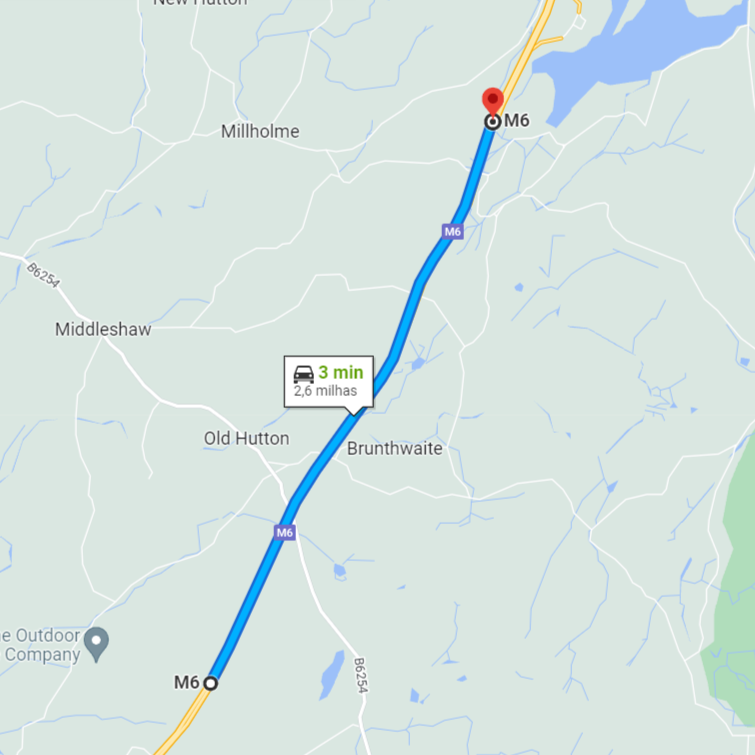
\includegraphics[width=6cm]{./img/mapaInglaterra.png} }}
    \caption{Figuras dos trechos escolhidos para a análise.}
\end{figure}

\subsection{Objetivos}

\qquad O objetivo era utilizar os dados extraídos do Kartaview para medir as distâncias percorridas pelo carro e a velocidade desse percurso. As distâncias deveriam ser calculadas por meio de 3 métodos de medição: fórmula de Haversine, projeção das coordenadas esféricas no plano e a trigonometria esférica. Depois de conseguir esses resultados, eles deveriam ser comparados com o resultado real, que poderia ser obtido por meio de sites, como o Google Maps ou com a análise de pontos fiduciais presentes nas imagens do percurso.

\subsection{Dados e métodos}

\qquad Foram utilizados os dados da API do Kartaview. O grupo decidiu produzir métodos em código que fossem capazes de acessar a API da plataforma e requisitar os dados diretamente, sem a necessidade de, por exemplo, extrair os dados manualmente com o Postman.

\quad Os dados são recebidos como um JSON, depois são filtrados para conter apenas as informações necessárias para os experimentos. As informações utilizadas são: latitude e longitude (para que seja possível calcular as distâncias), o index da foto (para saber a ordem), a url da foto (para poder baixá-la) e a data e horário (para saber a diferença de tempo entre as imagens).

\quad Além disso, o programa possui uma função que baixa da internet todas as imagens de um dado trajeto para que seja possível fazer a análise dos pontos fiduciais. No caso do trecho brasileiro, são 443 fotos amostradas e, no trecho Inglês, são 118 amostras.

\quad Para a parte de análise, as distâncias foram calculadas por meio dos 3 métodos e foram plotadas em um gráfico junto com a ``distância real" fornecida pelo sistema do Google Maps de medição e a variação dos pontos fiduciais.

\subsection{Resultados experimentais}

\subsubsection{Brasil}

\qquad Primeiramente, a distância calculada pelo Google Maps para o trajeto foi 7,5km e, analisando os pontos fiduciais, a distância encontrada foi 7,8km. As imagens a seguir mostram as placas da rodovia registradas nas fotos.

\begin{figure}[!h]
    \centering
    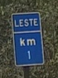
\includegraphics[width=1.5cm]{./img/BPlaca1.png}\quad
    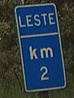
\includegraphics[width=1.5cm]{./img/BPlaca2.png}\quad
    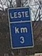
\includegraphics[width=1.5cm]{./img/BPlaca3.png}\quad
    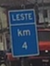
\includegraphics[width=1.5cm]{./img/BPlaca4.png}\quad
    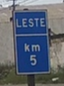
\includegraphics[width=1.5cm]{./img/BPlaca5.png}\quad
    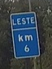
\includegraphics[width=1.5cm]{./img/BPlaca6.png}\quad
    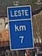
\includegraphics[width=1.5cm]{./img/BPlaca7.png}\quad
    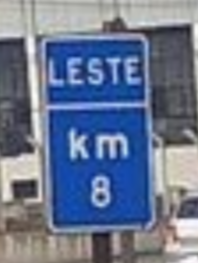
\includegraphics[width=1.5cm]{./img/BPlaca8.png}
    \caption{Imagem das placas do percurso no Brasil.}
\end{figure}

\qquad Depois da coleta dos pontos fiduciais e da distância medida pelo Maps, o programa de medição de distância foi rodado para que os 3 diferentes metros estimassem a distância. O primeiro teste media a distância total percorrida, gerando um gráfico de tempo por distância.

\qquad A princípio, foi percebido um comportamento estranho no gráfico. Por volta do primeiro minuto de trajeto, a distância estabilizou e só voltou a crescer por volta de um minuto e meio depois. Esse fato gerou desconfiança sobre o funcionamento do código, no entanto, ao analisar os dados, é possível ver que de fato essa pausa existiu no trajeto, no entanto, em vez do Kartaview tirar diversas fotos com o carro parado, ele percebeu esse não deslocamento e retirou as fotos paradas do registro. Assim, no momento da pausa, duas fotos consecutivas tiveram uma diferença de quase um minuto e meio, como pode ser visto a seguir no gráfico:


\begin{figure}[!h]
    \centering
    \subfloat[Imagem completa]{{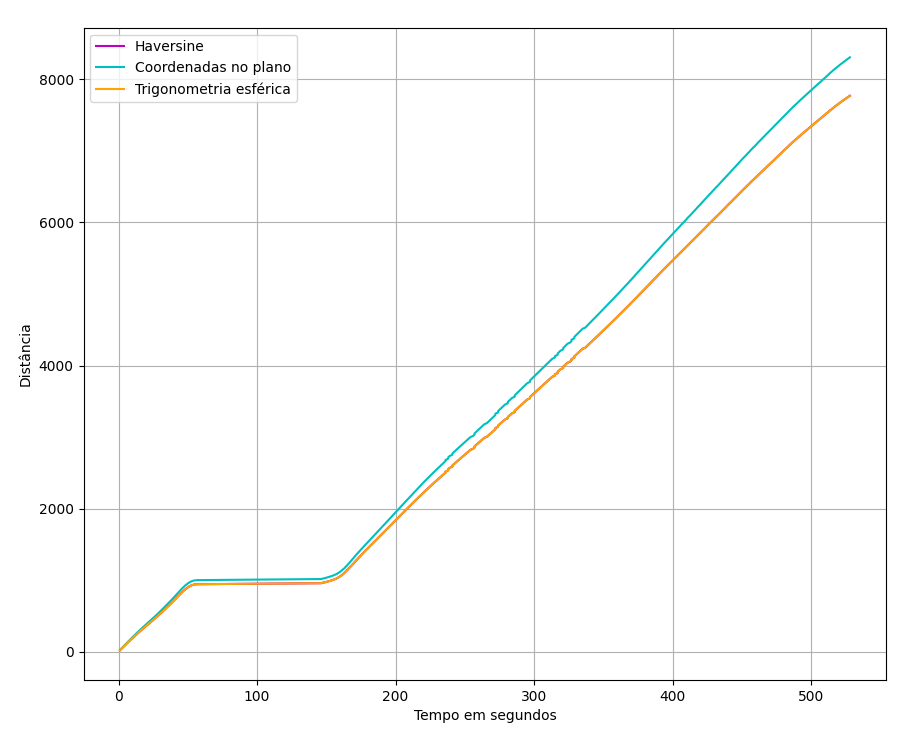
\includegraphics[width=8cm]{./img/grafico_distancia_acumulada.png}}}\quad
    \subfloat[Zoom da imagem]{{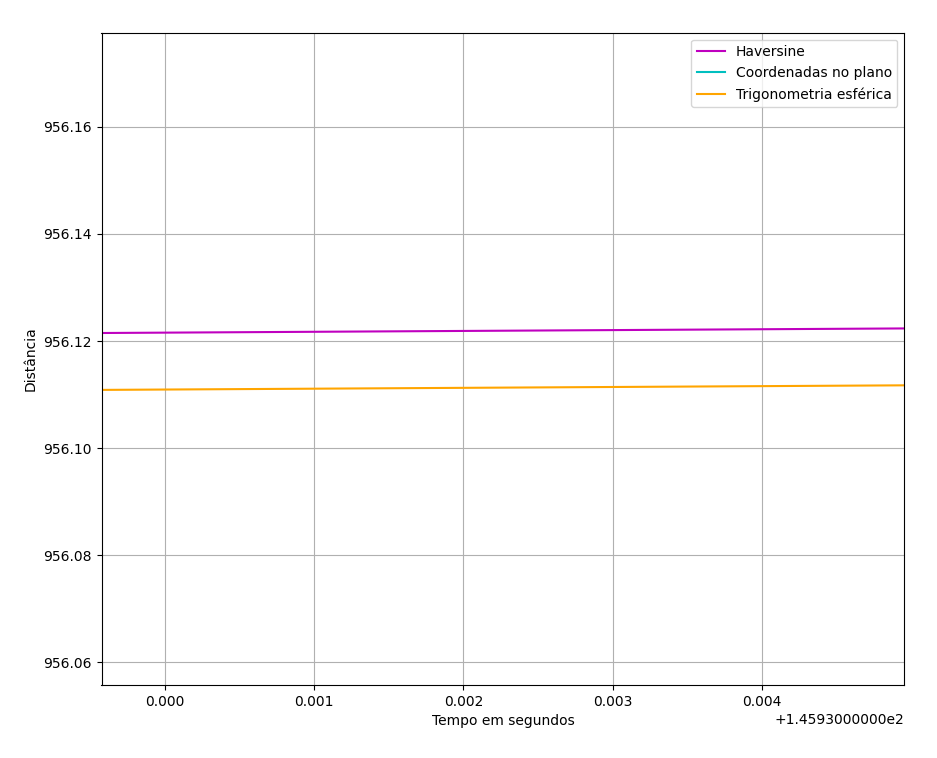
\includegraphics[width=8cm]{./img/grafico_distancia_acumulada_zoom.png}}}
    \caption{Gráfico da distância pelo tempo.}
\end{figure}

\qquad Outra coisa interessante, visível na segunda imagem, é que os métodos de Haversine e Trigonometria Esférica ficaram muito próximos, mesmo no final do trajeto, a diferença foi menor que 1 metro. No final das contas, o que divergiu mais foi o método de planificação da esfera. Os resultados dos trechos foram:

\vspace{0.5cm}

{\centering
\begin{tabular}{ | l | l | }
    \hline
    Método & Valor calculado (em metros)\\ \hline
    Coordenadas no plano & 8309.73 \\ \hline
    Haversine & 7771.52 \\\hline
    Maps & 7500.00 \\ \hline
    Pontos fiduciais & 7800.00 \\ \hline
    Trigonometria esférica & 7771.5 \\ \hline
\end{tabular}
\par
}

\vspace{0.5cm}

\qquad Como requisitado, o programa mede, entre cada par de pontos, a distância percorrida, o tempo, a velocidade etc, no entanto, colocar esses dados no relatório não seria tão ilustrativo. Por isso, o foco será no percurso completo. A distância já foi mostrada no gráfico anterior, a velocidade está no gráfico a seguir e o tempo do percurso foi de 8 minutos e 48 segundos, dos quais 1 minuto e 28 segundos o carro ficou parado.


\begin{figure}[!h]
    \centering
    \subfloat[Imagem completa]{{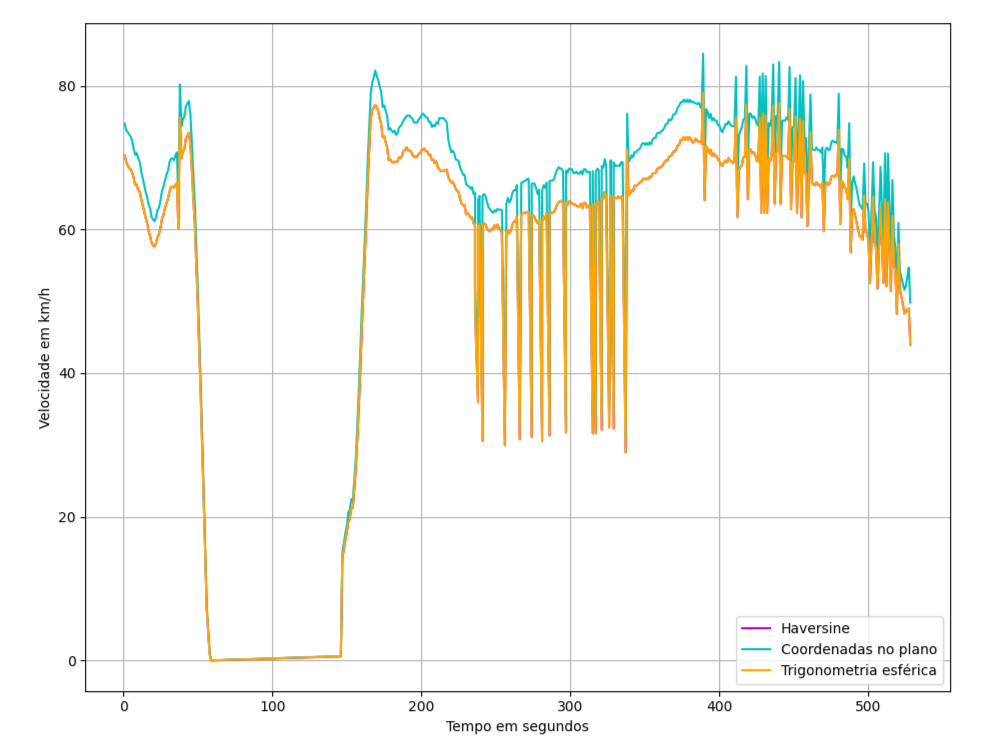
\includegraphics[width=8cm]{./img/grafico_velocidade_br.png}}}\quad
    \subfloat[Zoom da imagem]{{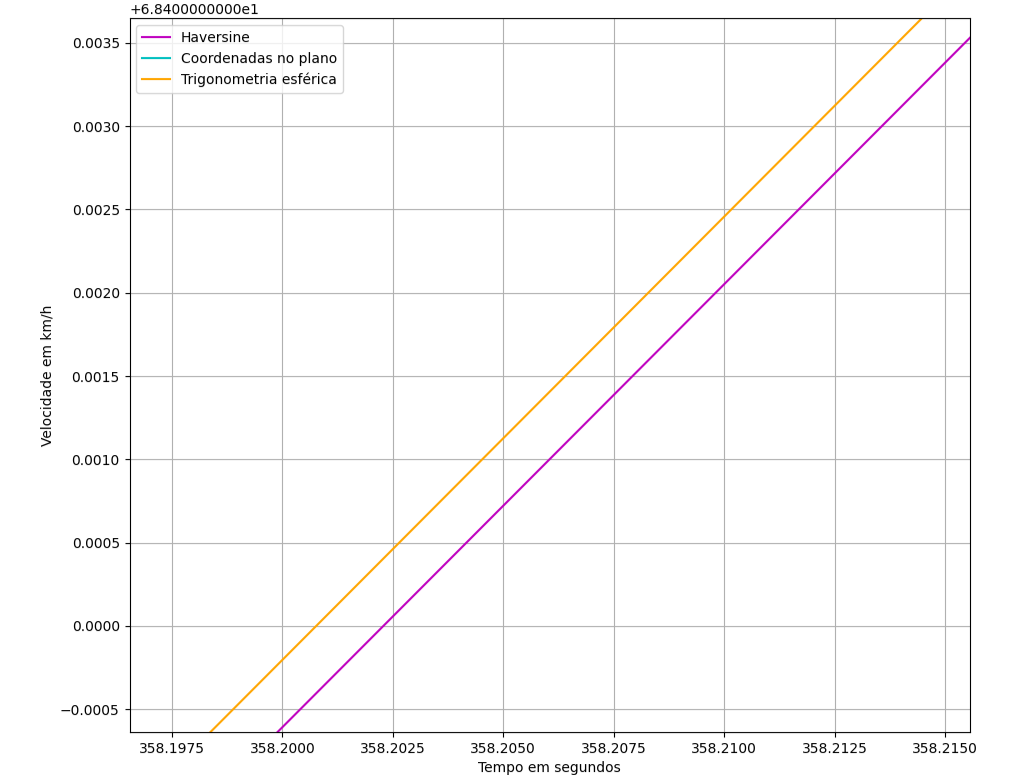
\includegraphics[width=8cm]{./img/grafico_velocidade_br_zoom.png}}}
    \caption{Gráfico da velocidade pelo tempo no percurso.}
\end{figure}





\subsubsection{Exterior}

\qquad No trecho do exterior, a distância calculada pelo Google Maps foi 2,6 milhas, ou seja 4,18km,  e, analisando os pontos fiduciais, a distância encontrada foi 4,2km. As imagens a seguir mostram as placas da rodovia registradas nas fotos.

\begin{figure}[!h]
    \centering
    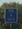
\includegraphics[width=1.5cm]{./img/IPlaca1.png}\quad
    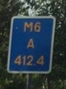
\includegraphics[width=1.5cm]{./img/IPlaca2.png}\quad
    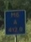
\includegraphics[width=1.5cm]{./img/IPlaca3.png}\quad
    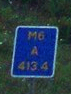
\includegraphics[width=1.5cm]{./img/IPlaca4.png}\quad
    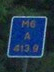
\includegraphics[width=1.5cm]{./img/IPlaca5.png}\quad
    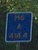
\includegraphics[width=1.5cm]{./img/IPlaca6.png}\quad
    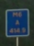
\includegraphics[width=1.5cm]{./img/IPlaca7.png}\quad
    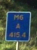
\includegraphics[width=1.5cm]{./img/IPlaca8.png}\quad
    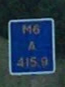
\includegraphics[width=1.5cm]{./img/IPlaca9.png}
    \caption{Imagem das placas do percurso na Inglaterra.}
\end{figure}

\qquad A tabela a seguir compila os resultados obtidos pelos diferentes métodos de medição:

\vspace{0.5cm}

{\centering
\begin{tabular}{ | l | l | }
    \hline
    Método & Valor calculado (em metros)\\ \hline
    Coordenadas no plano & 5029.66 \\ \hline
    Haversine & 4243.45 \\\hline
    Maps & 4180 \\ \hline
    Pontos fiduciais & 4200 \\ \hline
    Trigonometria esférica & 4243.45 \\ \hline
\end{tabular}
\par
}


\vspace{0.5cm}

\qquad Como requisitado, o programa mede, entre cada par de pontos, a distância percorrida, o tempo, a velocidade etc, no entanto, colocar esses dados no relatório não seria tão ilustrativo. Por isso, o foco será no percurso completo. O gráfico da distância e da velocidade estão no gráfico a seguir e o tempo do percurso foi de 2 minutos e 10 segundos.

\begin{figure}[!h]
    \centering
    \subfloat[Imagem completa]{{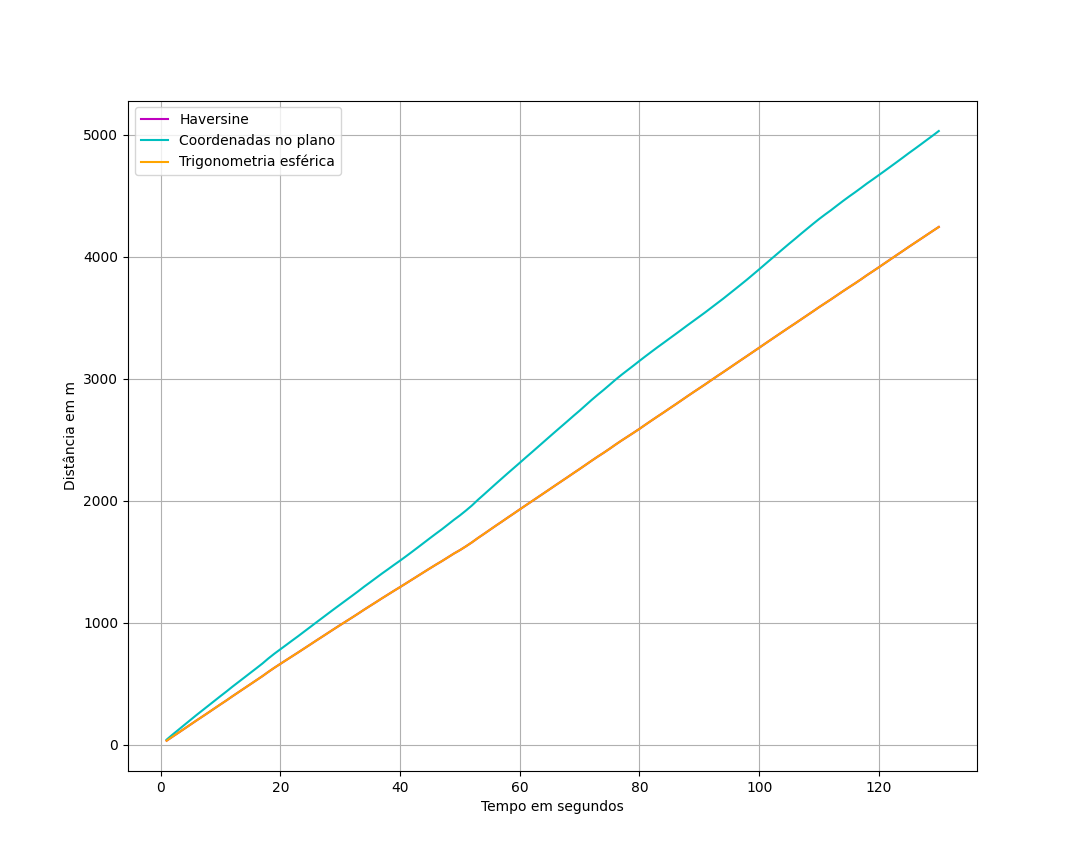
\includegraphics[width=7cm]{./img/grafico_distancia_acumulada_uk.png}}}\quad
    \subfloat[Zoom da imagem]{{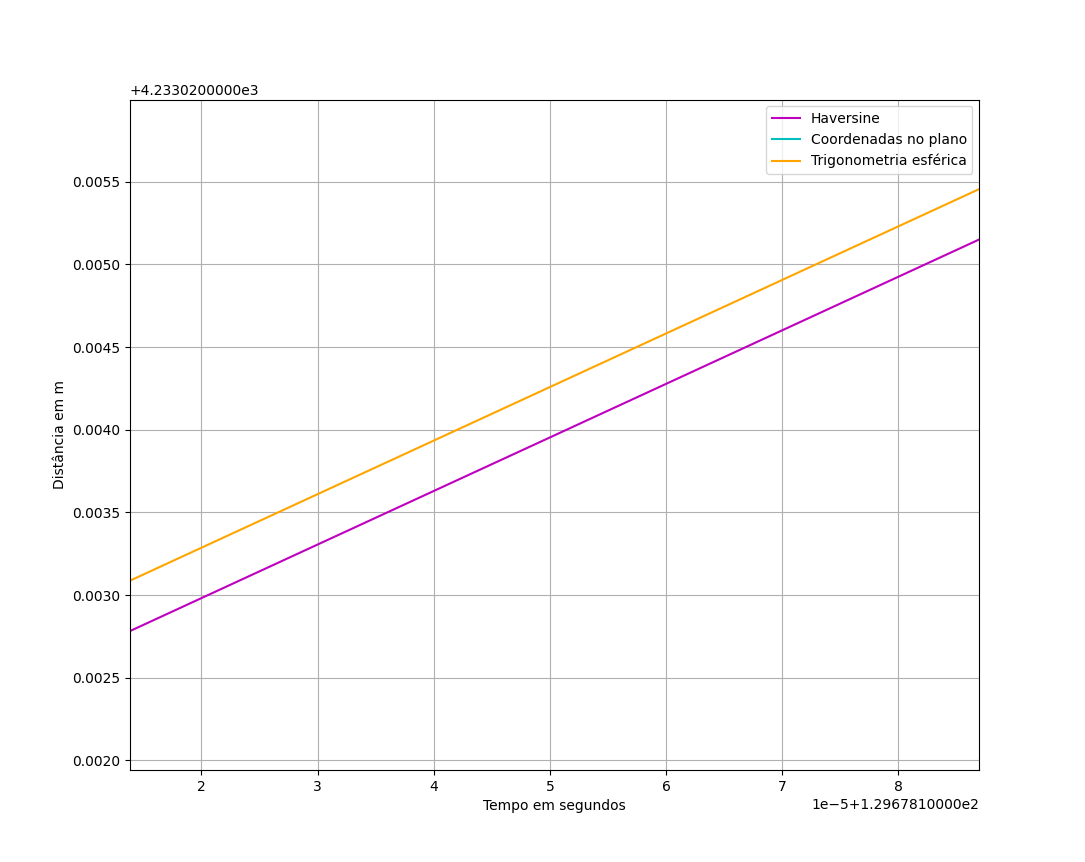
\includegraphics[width=7cm]{./img/grafico_distancia_acumulada_uk_zoom.png}}}
    \caption{Gráfico da distância pelo tempo no percurso.}
    
    \subfloat[Imagem completa]{{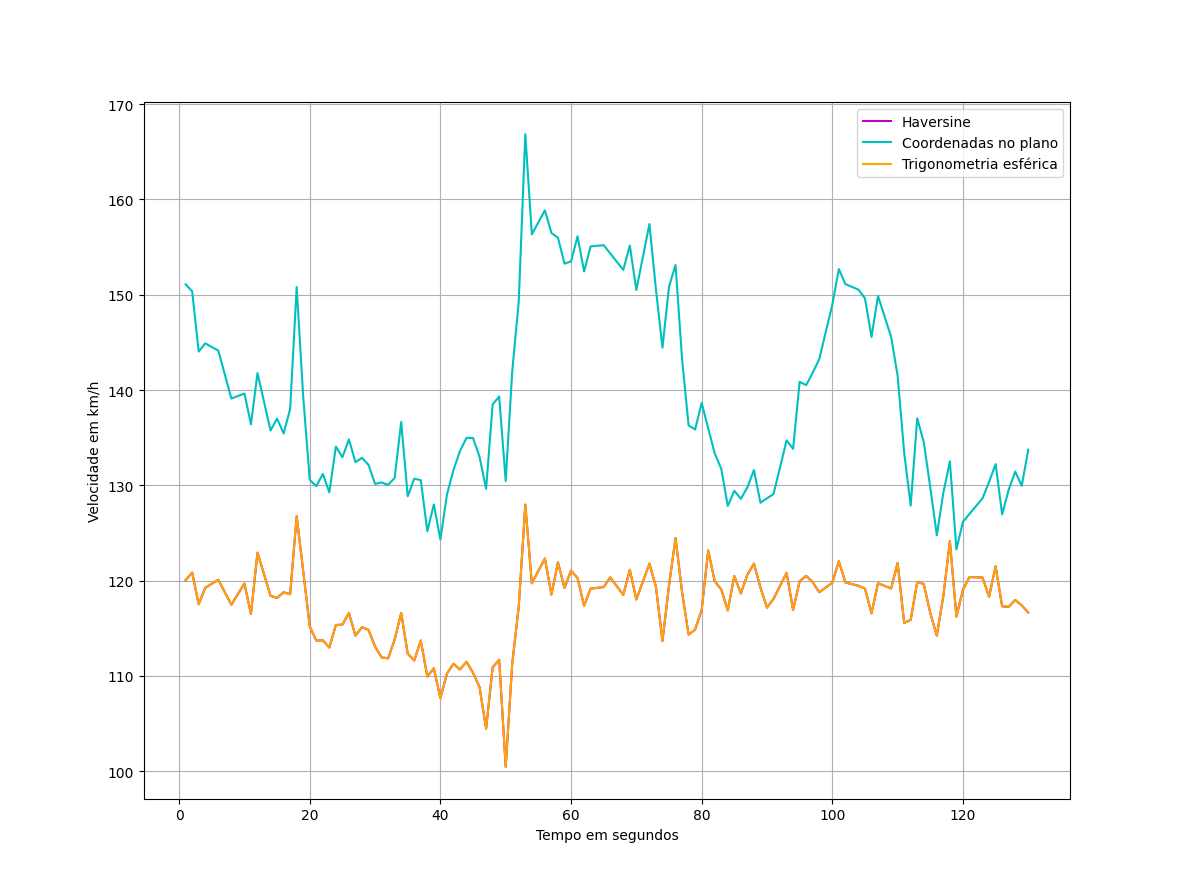
\includegraphics[width=7cm]{./img/grafico_velocidade_uk.png}}}\quad
    \subfloat[Zoom da imagem]{{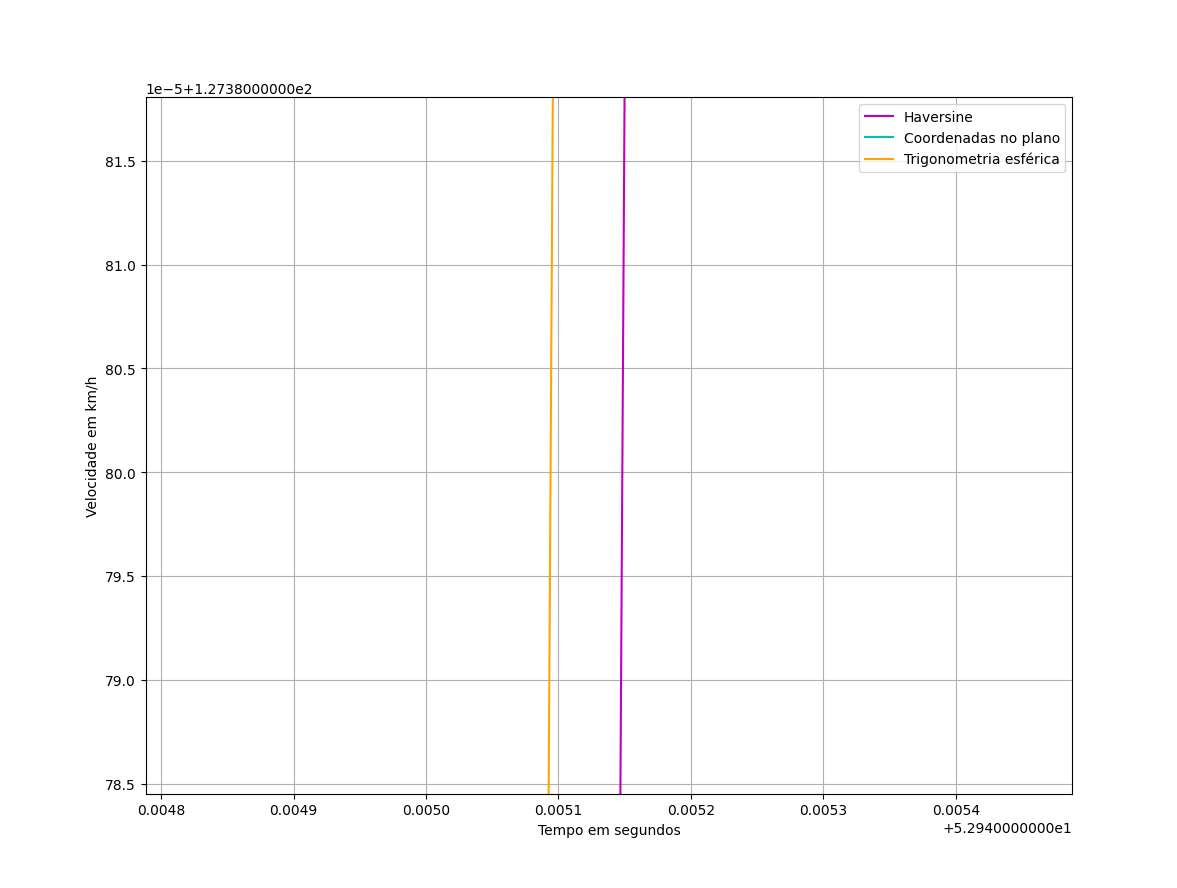
\includegraphics[width=7cm]{./img/grafico_velocidade_uk_zoom.png}}}
    \caption{Gráfico da velocidade pelo tempo no percurso.}
\end{figure}




\subsection{Discussão}

\qquad Os testes foram interessantes, pois foi possível ver quais métodos são mais precisos do que outros. Experimentar no Brasil e no exterior permite a reflexão e comparação dos métodos. Tanto no caso braisleiro, quanto no inglês, é visível que o pior método é o das coordenadas no plano, já que ele simplifica muito o cálculo da distância, tratando a superfície terrestre como algo 2D.

\qquad No caso dos outros dois métodos, que de fato consideram o formato geoide da Terra, os resultados foram igualmente excelentes. Os resultados calculados pelos métodos foram quase iguais aos vistos nos pontos fiduciais e no Google Maps. Nesse sentido, fica claro que usar um dos dois métodos (Haversine e Trigonometria Esférica) produzirá resultados melhores, provavelmente em todos os casos, já que o Brasil e o Reino Unido estão em latitudes e longitudes muito diferentes, mas os resultados foram muito precisos nos dois casos.

\qquad Quanto ao gráfico da velocidade, é possível ver que o caso inglês produziu um gráfico muito mais estável. Isso ocorreu, pois no caso braisleiro, as fotos foram tiradas em períodos muito curtos, de modo que ao analisar os dados, aparecem fotos nas quais a data e o horário, incluindo os segundos, são exatamente iguais. Dessa forma, qualquer pequena variação ou erro de medição de latitude e longitude, vai gerar linhas muito íngrimes de variação, pois o tempo é muito curto para o erro ser amortizado pelo tempo, como ocorreu no caso inglês.

\newpage

\section{Modelos de movimentos diversos (máximo de 4 páginas)}

\subsection{Introdução}

\qquad Inicialmente, foi necessário que o grupo escolhesse dois movimentos para modelá-los. Para este trabalho, os movimentos escolhidos foram o bloco de aço na rampa de madeira e o movimento circular. O programa deveria ter como entrada as condições iniciais do experimento, como a massa dos objetos envolvidos, a inclinação da rampa na qual o bloco iria deslizar etc. A partir dessas informações, o programa deveria simular o deslocamento do objeto seguindo as fórmulas de física vistas em aula.

\qquad Esse tipo de experimento é importante, pois é utilizado em diversas áreas da computação, como jogos, simuladores e programas educacionais. Por fim, os resultados do simulador foram comparados com os resultados dos experimentos feitos fisicamente por alunos do Instituto de Física da USP. 

\subsection{Objetivos}

\qquad O objetivo era extrair os dados experimentais disponíveis no site do IFUSP, organizá-los, em seguida, escrever dois simuladores para os movimentos circular e bloco na rampa, executá-los com as mesmas condições descritas nos experimentos do IFUSP e comparar os resultados simulados com os resultados experimentais. É desejável que no final, os resultados simulados estejam próximos aos experimentados. 


\subsection{Dados e métodos}

\qquad Os dados foram extraídos do site \url{http://www.fep.if.usp.br/~fisfoto/translacao/atrito/index.php} do Instituto de Física. Foi necessário extrair os dados de pelo menos 5 experimentos diferentes de cada tipo. Esses dados foram organizados em tabelas e as condições iniciais foram utilizados para simular o movimento pelo programa.

\subsubsection{Bloco na rampa}

\qquad Os dados extraídos são dos experimentos 1, 2, 4, 7 e 11 e estão tabelados a seguir:

\begin{figure}[!h]
    \centering
    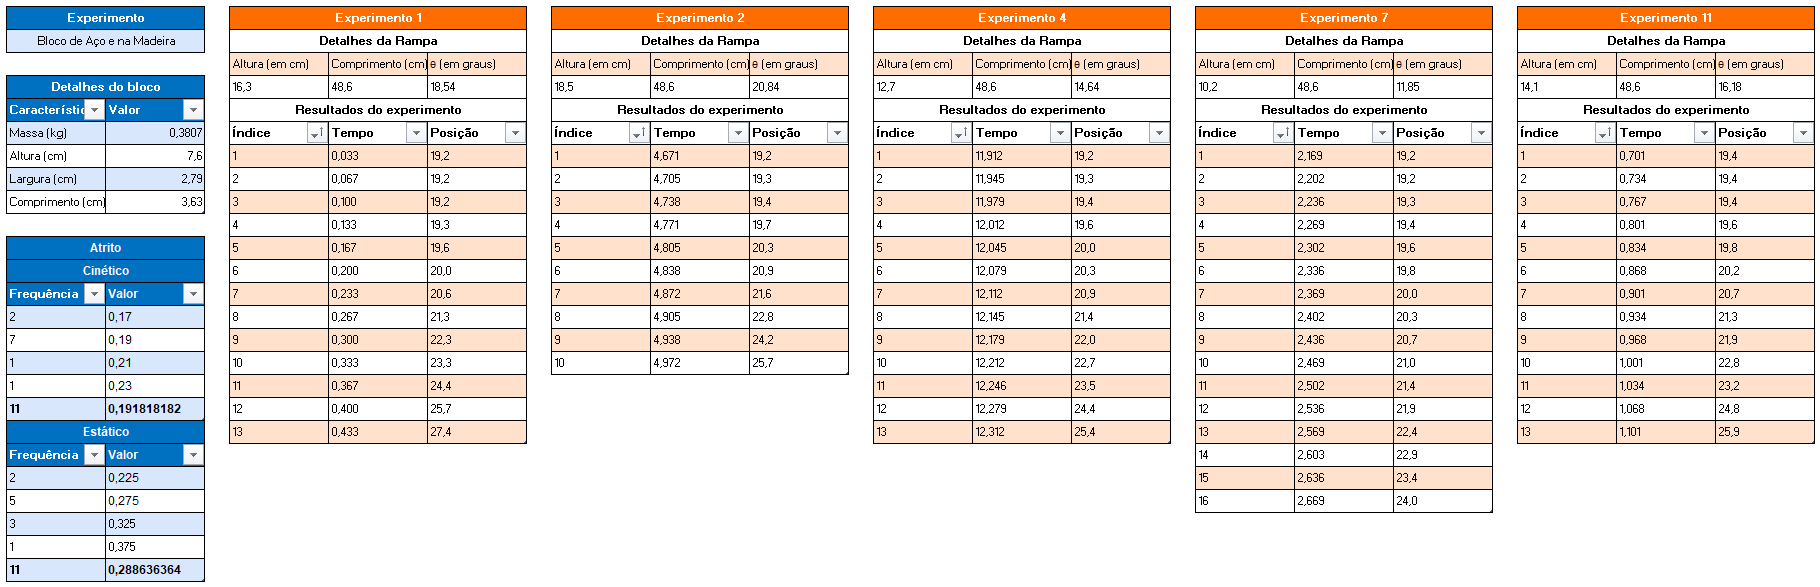
\includegraphics[width=16cm]{./img/tabelas_bloco_rampa.png}
    \caption{Dados do bloco na rampa.}
\end{figure}

\qquad O programa recebe a aceleração gravitacional, massa do bloco, coeficientes estático e cinético, velocidade e aceleração inicial do bloco, o ângulo da rampa, posição inicial, tempo inicial e final do experimento e o dt. Esses dados estão todos disponíveis na internet ou por meio do experimento, portanto, não foi difícil encontrá-los. Os coeficientes de atrito vieram do segundo documento disponível no site.



\subsubsection{Movimento circular}
\qquad Os dados extraídos são dos experimentos 2, 3, 5, 7 e 11 e estão tabelados a seguir:


\begin{figure}[!h]
    \centering
    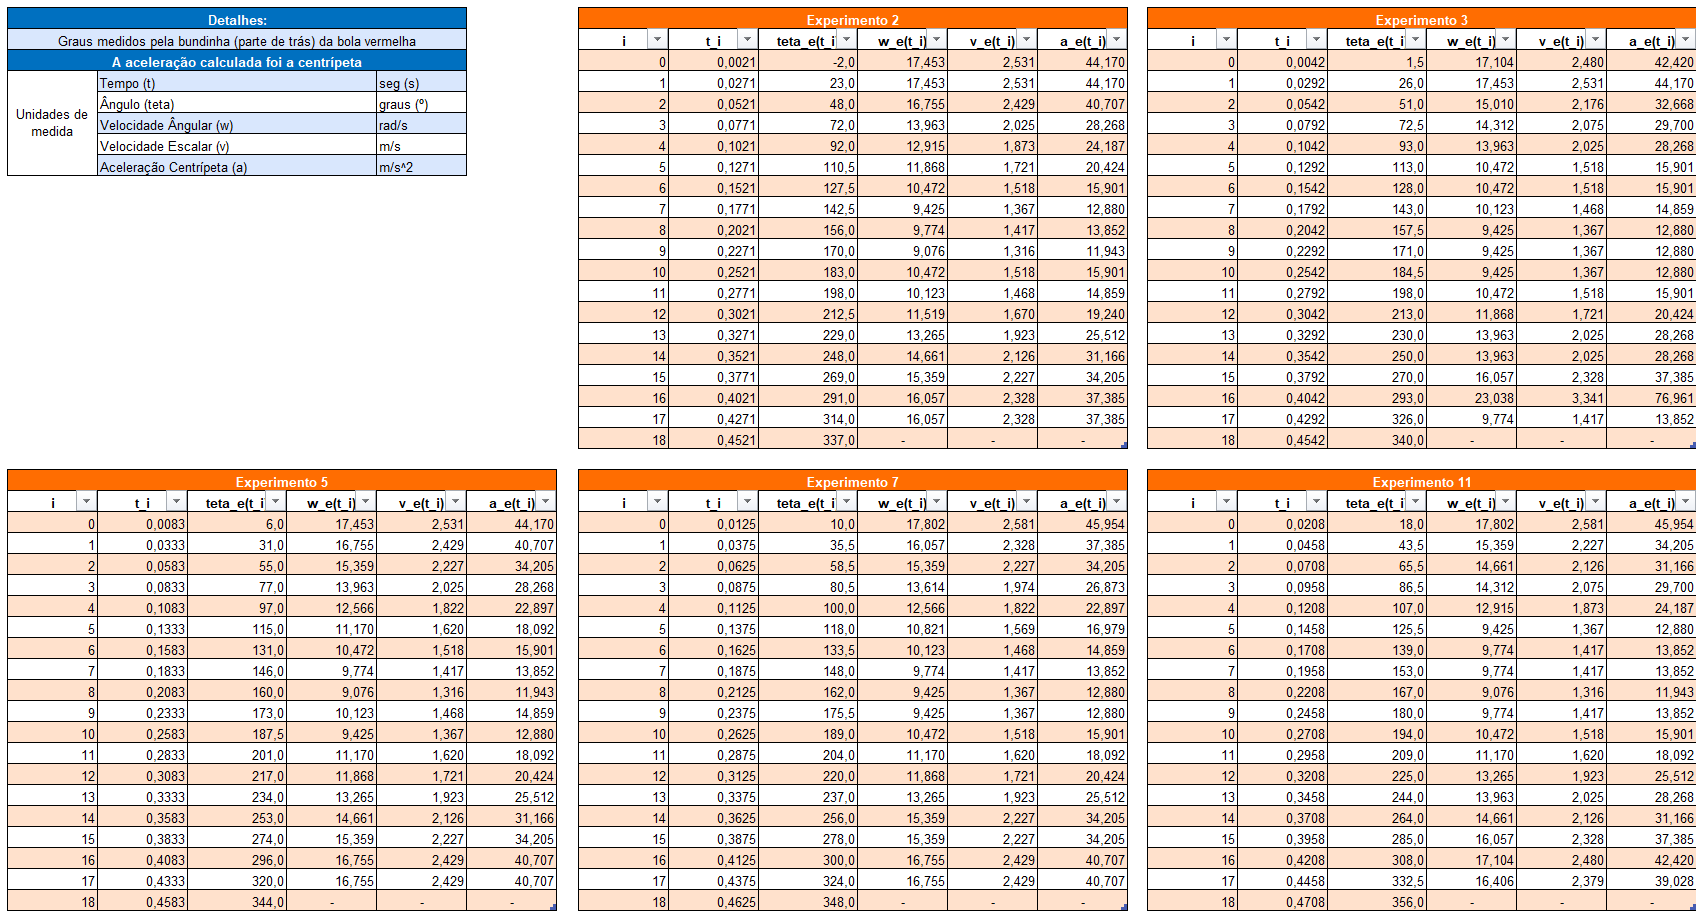
\includegraphics[width=16cm]{./img/tabelas_movimento_circular.png}
    \caption{Dados do movimento circular.}
\end{figure}


\qquad Explique os dados usados e os métodos desenvolvidos.

\subsection{Resultados experimentais}

\subsubsection{Bloco na rampa}




\begin{figure}[!h]
    \centering
    \subfloat[Experimento 1]{{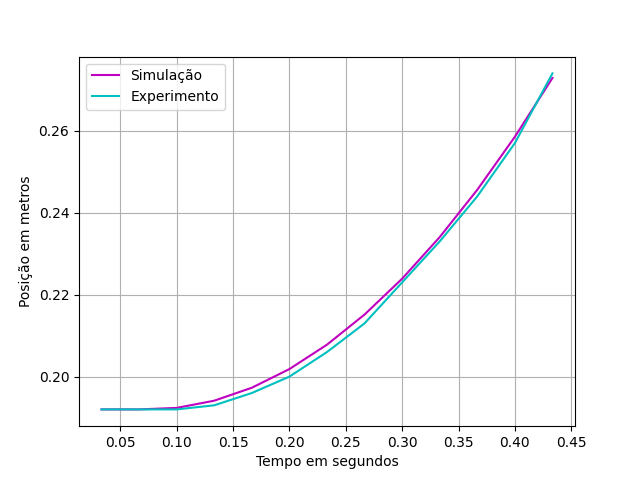
\includegraphics[width=5.25cm]{./img/bloco_rampa_1.png}}}\quad
    \subfloat[Experimento 2]{{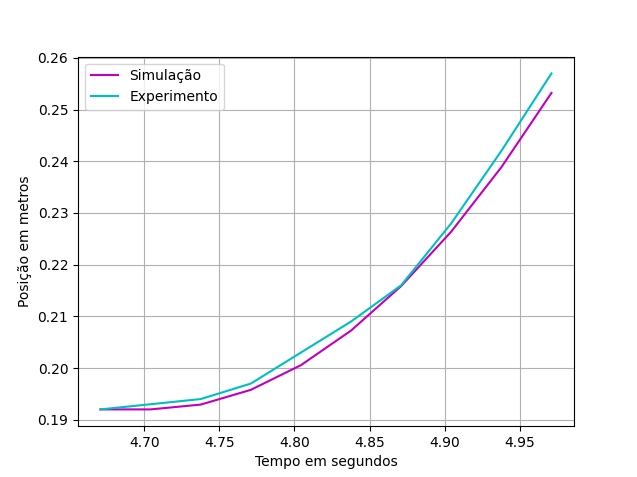
\includegraphics[width=5.25cm]{./img/bloco_rampa_2.png}}}\quad
    \subfloat[Experimento 4]{{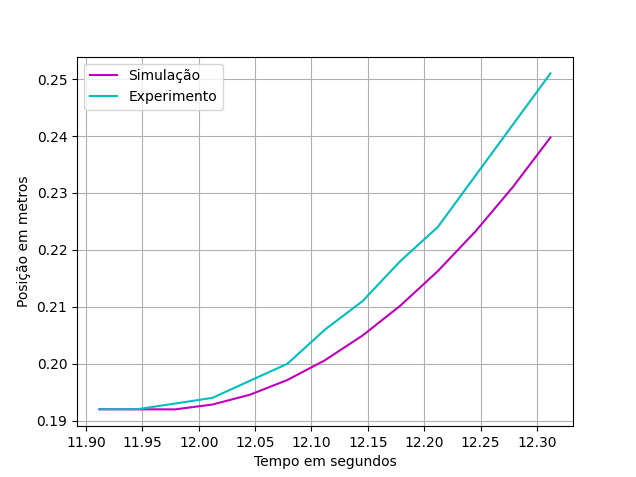
\includegraphics[width=5.25cm]{./img/bloco_rampa_4.png}}}\quad
    \subfloat[Experimento 8]{{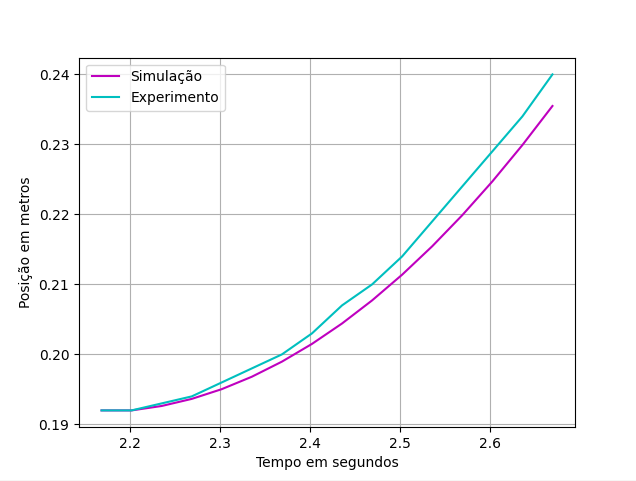
\includegraphics[width=5.25cm]{./img/bloco_rampa_8.png}}}\quad
    \subfloat[Experimento 11]{{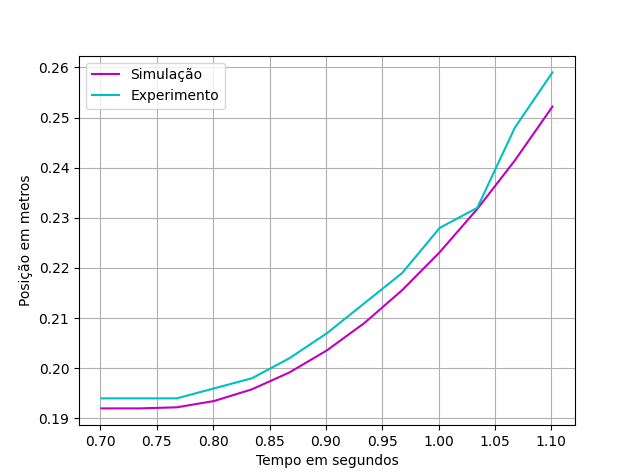
\includegraphics[width=5.25cm]{./img/bloco_rampa_11.png}}}
    \caption{Comparação entre a simulação e os dados experimentais.}
\end{figure}




\subsubsection{Movimento circular}

Apresente os resultados obtidos, Explore tabelas e gráficos ilustrativos.

\subsection{Discussão}

Interprete os resultados e apresente uma visão crítica.

\newpage

\section{Aplicação (máximo de 4 páginas)}

\subsection{Introdução}

Apresente uma introdução ao trabalho desenvolvido, fornecendo o contexto e a motivação.

\subsection{Objetivos}

Apresente o objetivo dessa parte do trabalho. Seja {\bf objetivo e claro}.

\subsection{Dados e métodos}

Explique os dados usados e os métodos desenvolvidos.

\subsection{Resultados experimentais}

Apresente os resultados obtidos, Explore tabelas e gráficos ilustrativos.

\subsection{Discussão}

Interprete os resultados e apresente uma visão crítica.

\end{document}